% --------------------------------------------------------------
% Basic LaTeX template for homework assignments.
% COMS W4701 - Artificial Intelligence
% --------------------------------------------------------------
\documentclass[11pt]{article}

\usepackage[margin=1in]{geometry}
\usepackage{amsmath,amsthm,amssymb}
\usepackage{tabularx}
\usepackage[T1]{fontenc}
\usepackage{enumerate}
\usepackage[]{forest}
\graphicspath{ {./img/} }

\forestset{.style={for tree=
{parent anchor=south, child anchor=north,align=center,inner sep=2pt}}}

\begin{document}

%           Your solutions start below this line
% --------------------------------------------------------------

\title{COMS W4119: Computer Networks\\
       Homework 2}
\author{Jackson Chen (jc4697)} % replace with your name and UNI
\maketitle

\section*{Network Applications \& Socket Programming}
  \begin{enumerate}[(a)]
    \item
      The two predominant modern application architectures are client-server
      and peer to peer.
    \item
      Client-server features an always on host that clients communicate with and
      receive resources from. There is no direct client to client interaction,
      as the server would handle the communication. This system is not auto-scaling,
      as hosts can be overwhelmed as more clients come online.

      Peer to peer has no always on server, so peers directly request resources
      from other peers and provides resources in return. This system is self-scaling,
      as more peers create more capability.
    \item
      Alice has both a client and server process, the client to download the movie
      from Bob, and a server process to upload chunks to other peers.

      If Bob isn't downloading anything, then he just has a server process running
      to send the movie to Alice. If he is downloading files, then he would have both
      processes (same logic as Alice above).
    \item
      \begin{enumerate}
        \item
          No, because he needs the port number that her application is running
          on her machine.
        \item
          TSL/SSL should be implemented in the application layer. She should use
          the SSL socket API or an SSL library that communicates with the TCP protocol.
      \end{enumerate}
    \item
      \begin{enumerate}
        \item
          Each socket is used for a bidirectional communication channel between a
          client and the server. A socket is needed for the server process to
          listen for clients. Then additional sockets are needed for the TCP server
          to handle any additional number of clients.
        \item
          There must be $n+1$ sockets for the TCP server.
        \item
          UDP does not support connections between clients and servers, thus
          no handshaking is needed. A UDP server just needs a single socket
          that can accept and handle multiple connections.
      \end{enumerate}
    \item
      \begin{enumerate}[(i)]
        \item
          A ``Connection Refused'' error occurs when running the TCPClient process
          first before running the TCPServer process. This happens because the client
          is unable to receive a handshake (and thus establish a connection) with
          a TCP server, as it is not running.
        \item
          The same ``Connection Refused'' error occurs for the same reason (the
          client is unable to receive a handshake from the server and this fails
          to establish a connection)
        \item
          No errors occur, but the server does not receive the message. This is
          because server is not running when the client unreliably sends the
          message, and is thus unable to receive it. No errors occur (unlike
          in the TCP case), since the client does not actually establish a connection
          via a handshake.
        \item
          The server receives the message sent by the client. In this situation,
          the server happened to be online as the message was being unreliably
          sent by the client.
        \item
          A ``Connection Refused'' error occurs because a server process runs on
          a unique combination of an IP and port number, and thus sending a
          TCP connection request to the wrong port number will fail to deliver
          a connection request to the server process.
        \item
          No error occurs (since no handshaking is necessary), but the message
          fails to be delivered to the server, since again the server process
          is uniquely identified by an IP and port number, and so sending the
          message to the wrong port will not send it to the server process.
      \end{enumerate}
  \end{enumerate}

\section*{The Web and HTTP}
  \begin{enumerate}[(a)]
    \item
      Non-persistent HTTP with a single TCP connection will require 11 total
      TCP connections to be established sequentially.

      The RTT will be:
      \[ \frac{3 * 10^7}{3 * 10^8} = 0.1 \text{ seconds} \]

      To establish a single TCP connection, three control messages are exchanged
      between the client and server. Since the control messages are 2000 bits,
      it will take $0.002$ seconds to fully transmit one control message, and thus
      $0.006$ seconds to transmit all the bits to establish the TCP connection.

      To send one 100 kBit object back to the client, it will take $0.1$ seconds.

      Thus to establish one TCP connection and send one object, it will take:
      \[ 2 * \text{RTT} + 0.006 + 0.1 = 0.306 \text{ seconds} \]

      Thus, in order to send all 11 objects from the server:
      \[ 11 * 0.306 = \boxed{3.366 \text{ seconds}} \]
    \item
      A TCP connection needs to be initiated to retrieve the the first downloaded
      object, and then the client has access to the references to the other ten
      objects, and can thus establish 10 connections in parallel.

      The RTT is still $0.1$ seconds, and the time to transmit the control messages
      per TCP connection is $0.006$ seconds.

      To transmit the initial 100 kBit object in the first TCP connection, it will take
      $0.1$ seconds. Thus, the time to establish the first TCP connection is:
      \[ 2 * \text{RTT} + 0.006 + 0.1 = 0.306 \text{ seconds} \]

      To send the remaining ten 100-kBit objects in parallel, it would be equivalent
      to sending 1 million bits through the link at once, and thus take $1$ second
      to fully transmit the 10 objects.

      Because the client would send out 10 control messages simultaneously to
      establish 10 parallel connections, the client would be sending out
      $2000 * 10 = 20 \text{ Kbits}$ through the link, which would take
      $0.02$ seconds, and thus $0.06$ seconds to establish the 3-way handshake
      across all ten simultaneous connections.

      The time to establish parallel TCP connections and transmit the next ten objects
      is:
      \[ 2 * \text{RTT} + 0.06 + 1 = 1.26 \text{ seconds} \]

      The time to retrieve all 11 objects is just:
      \[ 0.306 + 1.26 = \boxed{1.566 \text{ seconds}} \]
    \item
      When using a persistent HTTP, the propagation delay will be $2 * \text{RTT}$
      to retrieve the first object (since it needs to set up the TCP connection),
      but then drop to $1 \text{RTT}$ for the remaining file transmissions.

      From part (a), establishing and transmitting the first object takes
      $0.306$ seconds.

      Transmitting the remaining objects will individually take:
      \[ \text{RTT} + 0.002 + 0.1 = 0.202 \text{ seconds} \]
      Note the $0.002$ instead of $0.006$, this is because only one control message
      needs to be sent from the client to the server.

      Thus, the total time it takes to get 11 objects using persistent HTTP is:
      \[ 0.306 + 10 * 0.202 = \boxed{2.326 \text{ seconds}} \]
    \item
      The gains are decent (but not by orders of magnitude), as it shaved off $1.04$
      seconds, or around 30 percent of the total time.
    \item
      If the link length is $3 * 10^{10}$ meters, then the RTT would be 100 seconds,
      which would make using persistent HTTP significant more efficient by orders of
      magnitude as it cuts down on one RTT, or 100 seconds, for every object retrieved.
    \item
      When Jeff first visits Amazon, Amazon's server creates a unique ID for Jeff,
      stores it in a database, and then sets a cookie in Jeff's client to store
      his unique ID. This way next time Jeff visits Amazon, his browser sends the
      cookie with his unique ID to the Amazon server, which is able to retrieve
      Jeff's latest session from the database.
    \item
      Different devices and browsers are different clients, and thus cookies stored in one
      client are not accessible from another.
    \item
      As the video was being streamed for the first time, it was being cached in a
      proxy server (with a faster transmission speed). This made a later retrieval
      much faster for Jeff.
    \item
      The cache hit rate is just the complement of the access link utilization
      rate, thus $1 - 0.45 = \boxed{0.55}$
    \item
      Because the transmission delay from the cache servers are negligible compared
      to the delay from the origin servers, the total delay is entirely comprised
      of the access link utilization multiplied by the delay from origin servers:
      \[ 0.45 * \text{RTT} = \boxed{0.45 \text{ seconds}} \]
  \end{enumerate}

\section*{Developer Tools and the Web}
  \begin{enumerate}[(a)]
    \item
      www.ee.columbia.edu
    \item
      files/seasdepts/clg2168@columbia.edu/person/person\_images/ethanKatzBassett.png
    \item
      The browser is requesting a persistent connection because of the field:
      \texttt{Connection: Keep-Alive}
    \item
      128.59.64.28
    \item
      The persistent TCP connection should be held open for a minimum of 5 seconds,
      and support a maximum of 99 requests from this connection before closing
      the connection.
    \item
      128.59.105.24
    \item
      The request URL of \texttt{https://www.columbia.edu/} sends a GET request for
      the HTML file, because the response header from the server has the field:
      \texttt{Content-Type: text/html}
    \item
      The response status code is \texttt{304 Not Modified}, and it is returned when
      a cached copy of the file is up to date with the server.
  \end{enumerate}

\section*{Video Streaming and CDN}
  \begin{enumerate}[(a)]
    \item
      Stored video streaming services want to interact with the client to provide
      a seamless streaming experience as a user's bandwidth fluctuates
    \item
      Rather than directly implementing TCP, QUIC reduces the time it takes
      to set up a connection (by reducing the number of RTT's), and also doesn't
      block multiple resources if one resource loses packets along the way.
      \footnote{https\://en.wikipedia.org/wiki/QUIC\#QUIC}
    \item
      The server offers a manifest file that provides resource locations for
      different chunks so that the client is able to retrieve the correct chunk
      based on the resolution that it has decided to stream at.
    \item
      If the chunks are a fixed size, the client has less flexibility in
      adjusting the resolution that it is fetching in case if the bandwidth changes
      in the middle of downloading a specific chunk.

      If the video is divided into a fixed number of chunks, then the client could ensure that each chunk takes roughly the same time to download, and thus could
      adjust resolution much more consistently.
    \item
      31 GET requests: One for the HTML page and 30 for each of the chunks.
    \item
      DNS allows a service to connect the client to the closest, highest bandwith
      CDN server storing the object that the client is requesting, without the client
      needing to intervene.
    \item
      Yes, we can tell the Youtube server Bob is connect to is not in North America.

      Speed of light is $3 * 10^8 m/s$, thus the amount of time it takes for data
      to traverse an undersea ocean fiberoptic cable roundtrip is:
      \[ 2 * \frac{1 * 10^7 m}{3 * 10^8 m/s} = .066 s = 66 ms \]

      Thus it takes at least 66 milliseconds to traverse the transcontinental
      cables, and the fact that Bob's computer shows a ping less than that means
      the request cannot be travelling transcontinent.
    \item
      We cannot tell in this situation since there are several factors that could
      contribute to the slow RTT beyond just propagation delay: for example network
      congestion via queueing delay could be a factor.
    \item
      A records for \texttt{www.netflix.com} \\
      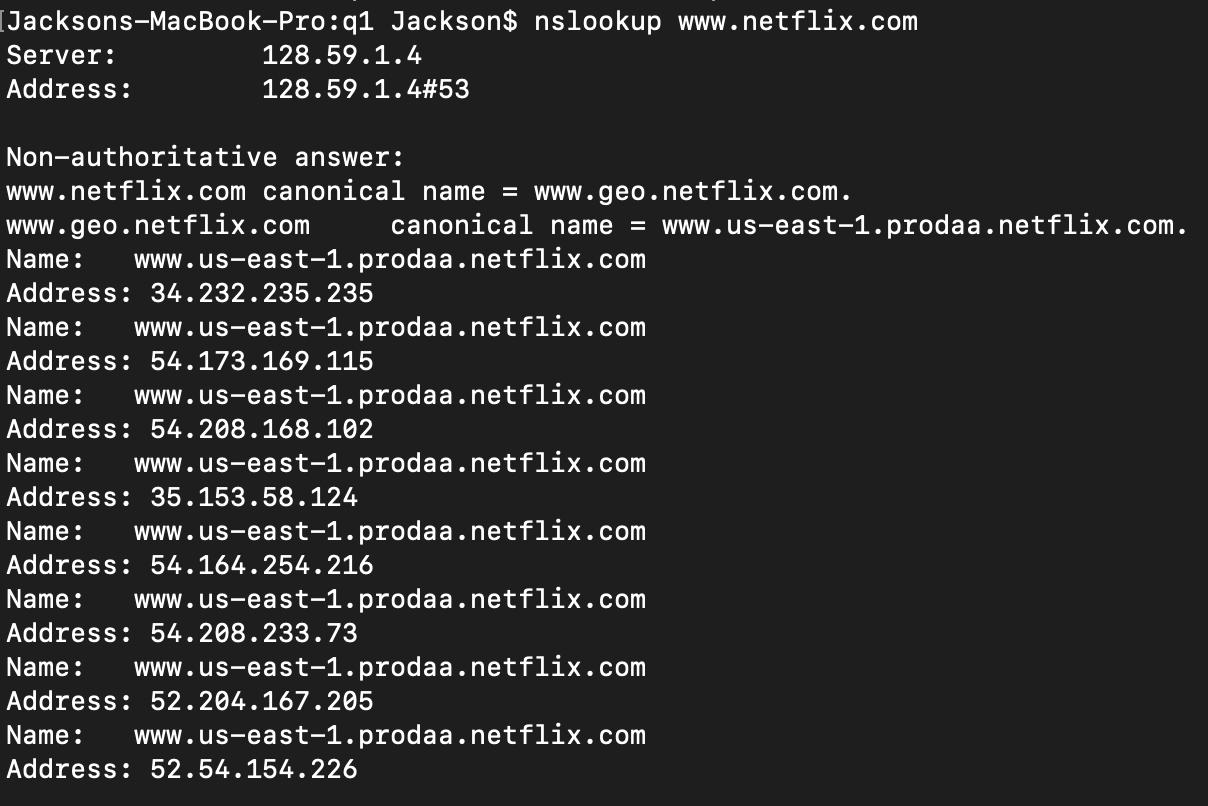
\includegraphics[width=15cm]{1}

      A records for \texttt{ipv4-c001-lga001-nysernet-isp.1.oca.nflxvideo.net } \\
      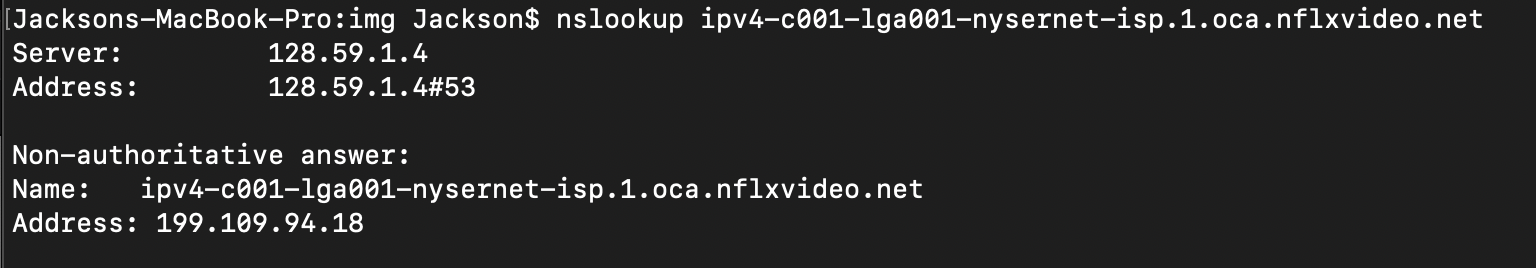
\includegraphics[width=15cm]{2}

      A records for \texttt{ae.nflximg.net} \\
      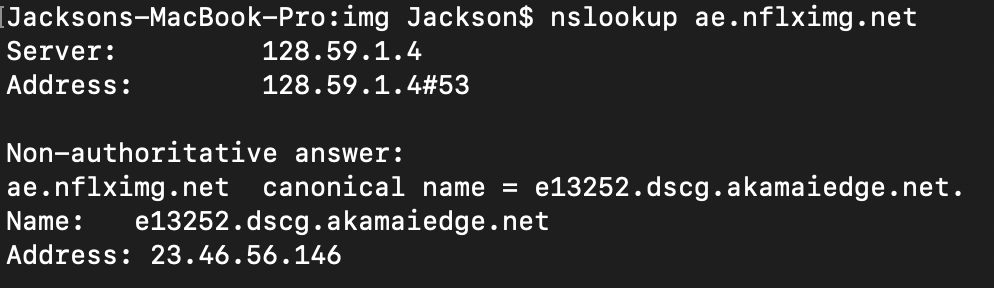
\includegraphics[width=15cm]{3}
    \item
      The hostname of \texttt{128.59.64.28} \\
      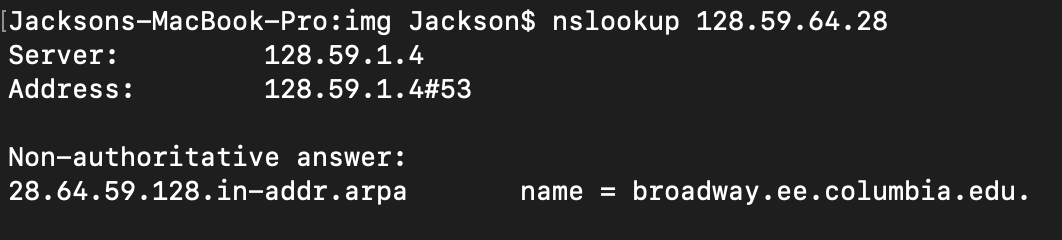
\includegraphics[width=15cm]{4}
    \item
      \texttt{nslookup} for the IP address does not return \texttt{www.netflix.com},
      this is because AWS servers handle requests from that hostname. \\
      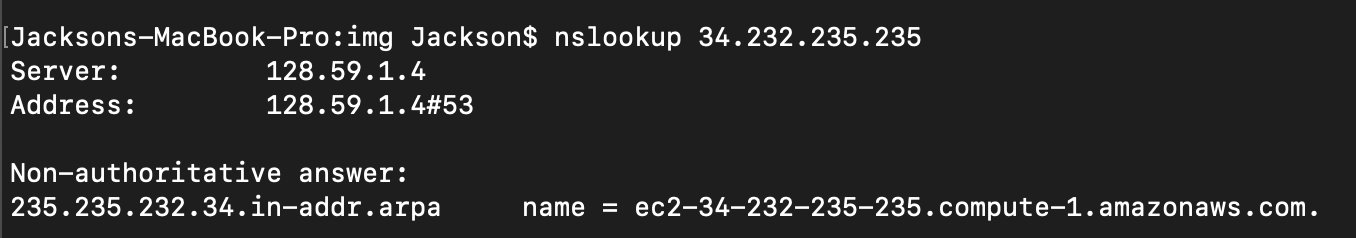
\includegraphics[width=15cm]{5}
    \item
      No, because NYSernet, an education focused ISP that provides internet for Columbia,
      is handling video chunk streaming for Netflix for the Columbia network. \\
      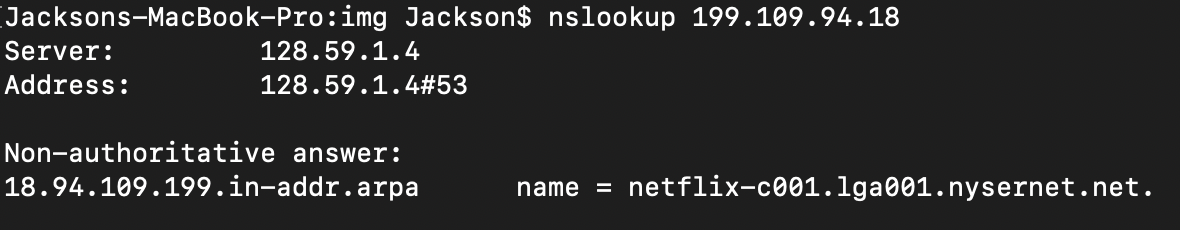
\includegraphics[width=15cm]{6}
    \item
      No because Akamai, a CDN provider, handles image resource delivery for Netflix. \\
      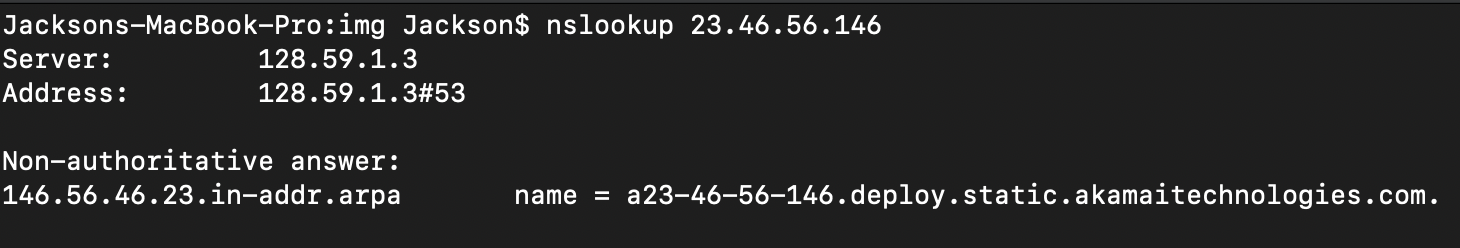
\includegraphics[width=15cm]{7}
    \item
      In Seattle, the IP address is 99.86.35.22 \\
      In New York, the IP address is 99.84.46.77 \\

      These two IP addresses are different because Amazon has different servers
      that handle requests in different geographic regions to minimize overall
      delay.

      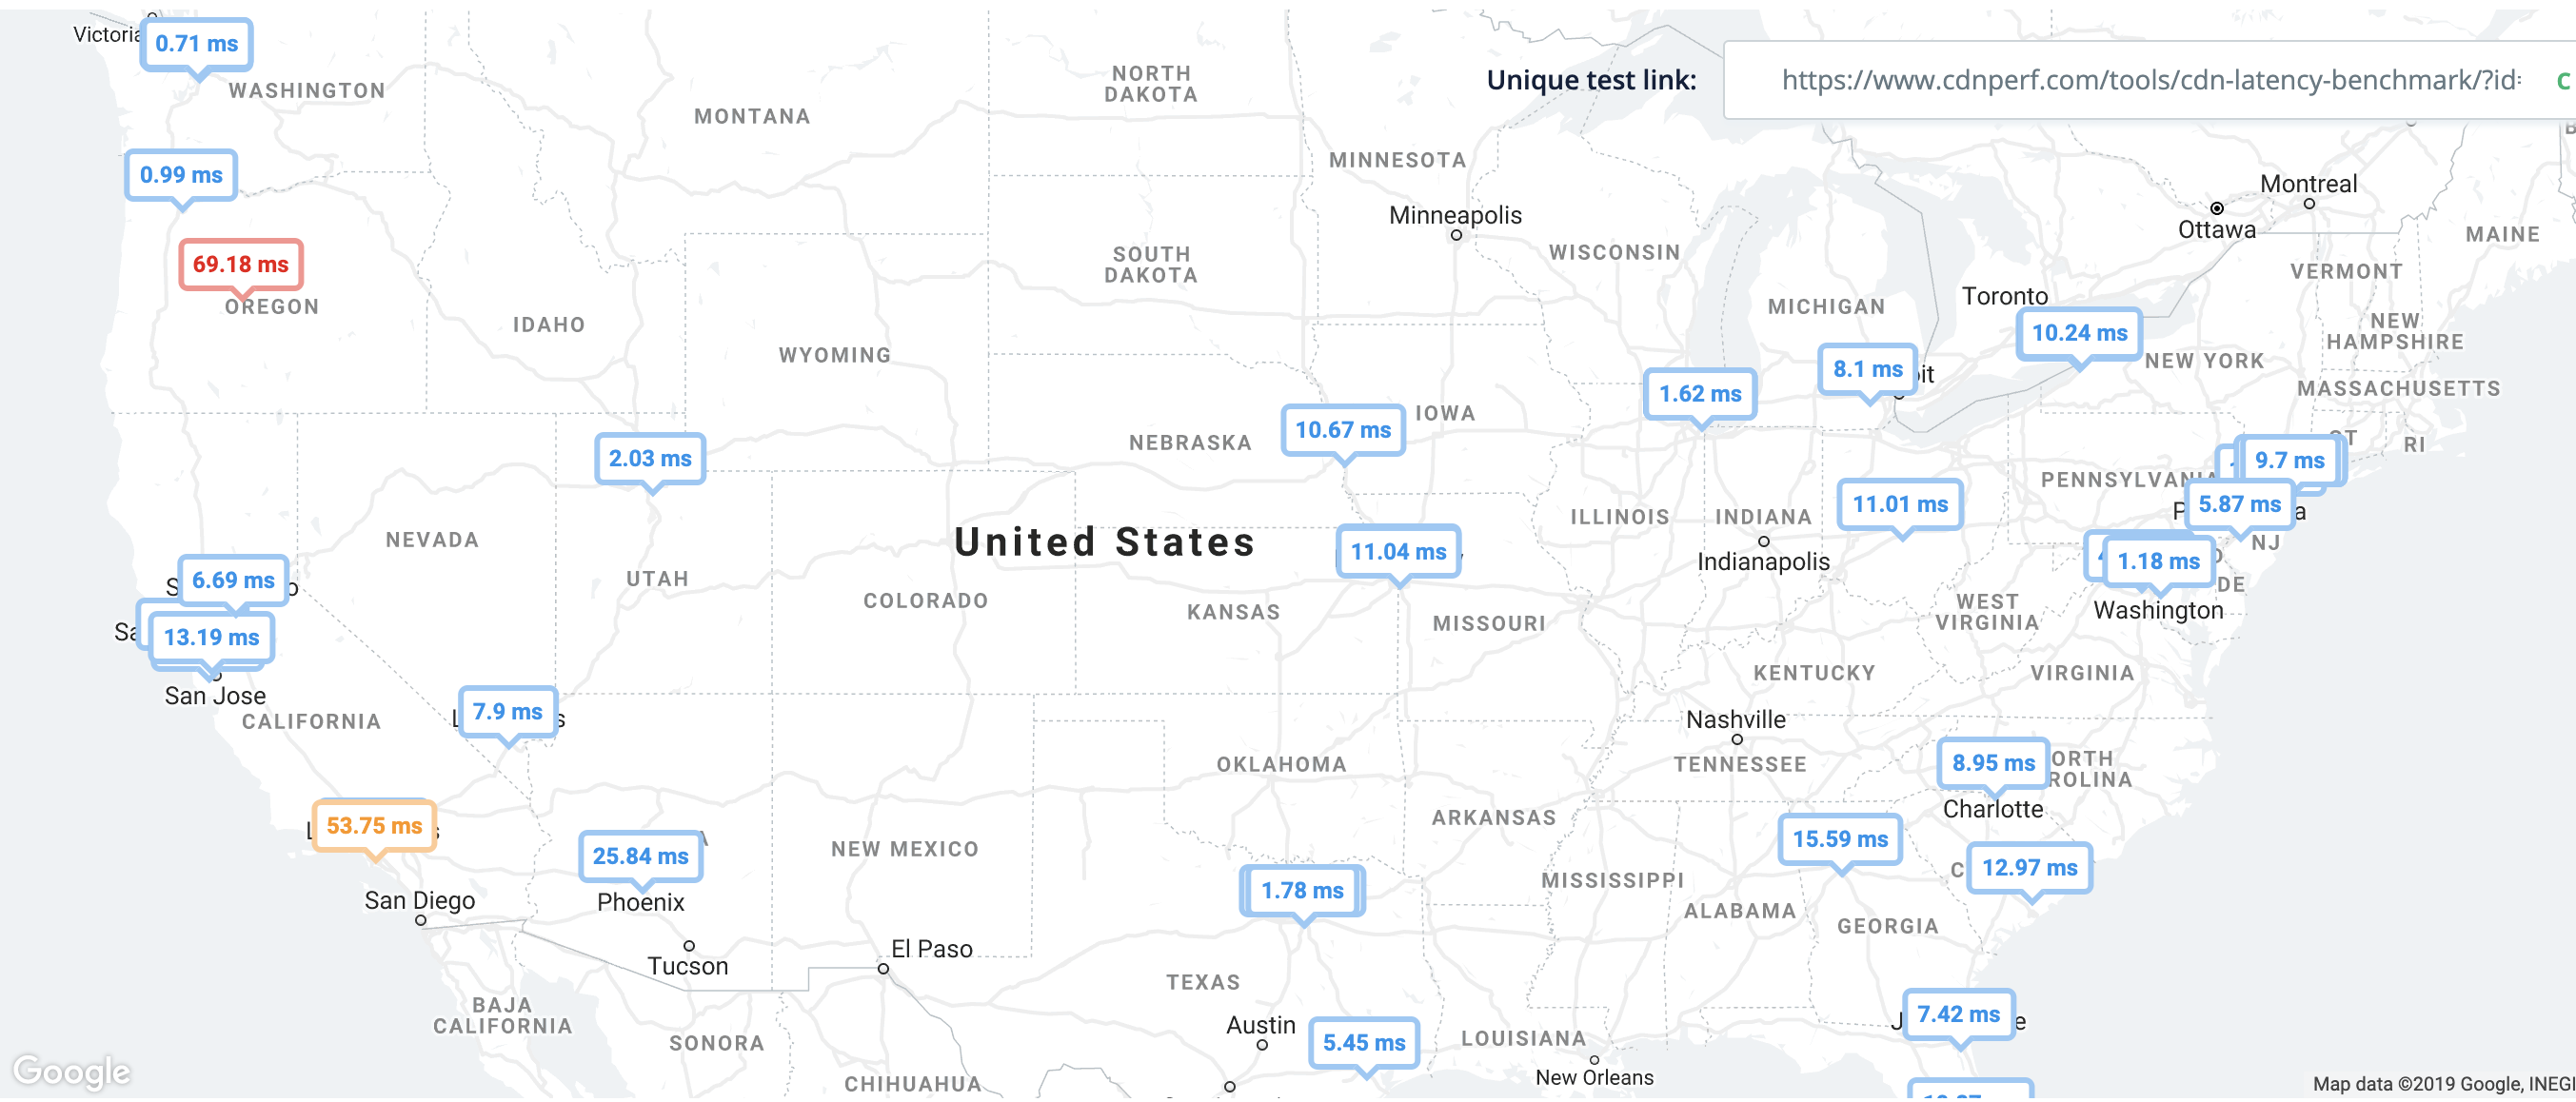
\includegraphics[width=15cm]{8} \\
      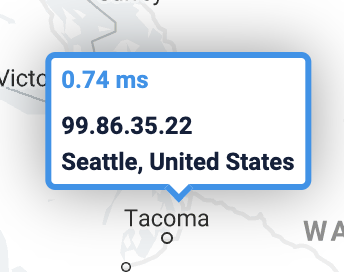
\includegraphics[width=15cm]{9} \\
      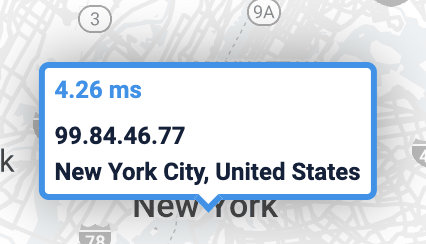
\includegraphics[width=15cm]{10}
    \item
      The server 99.86.35.22 is most likely in the Seattle region based on the ping
      map: \\
      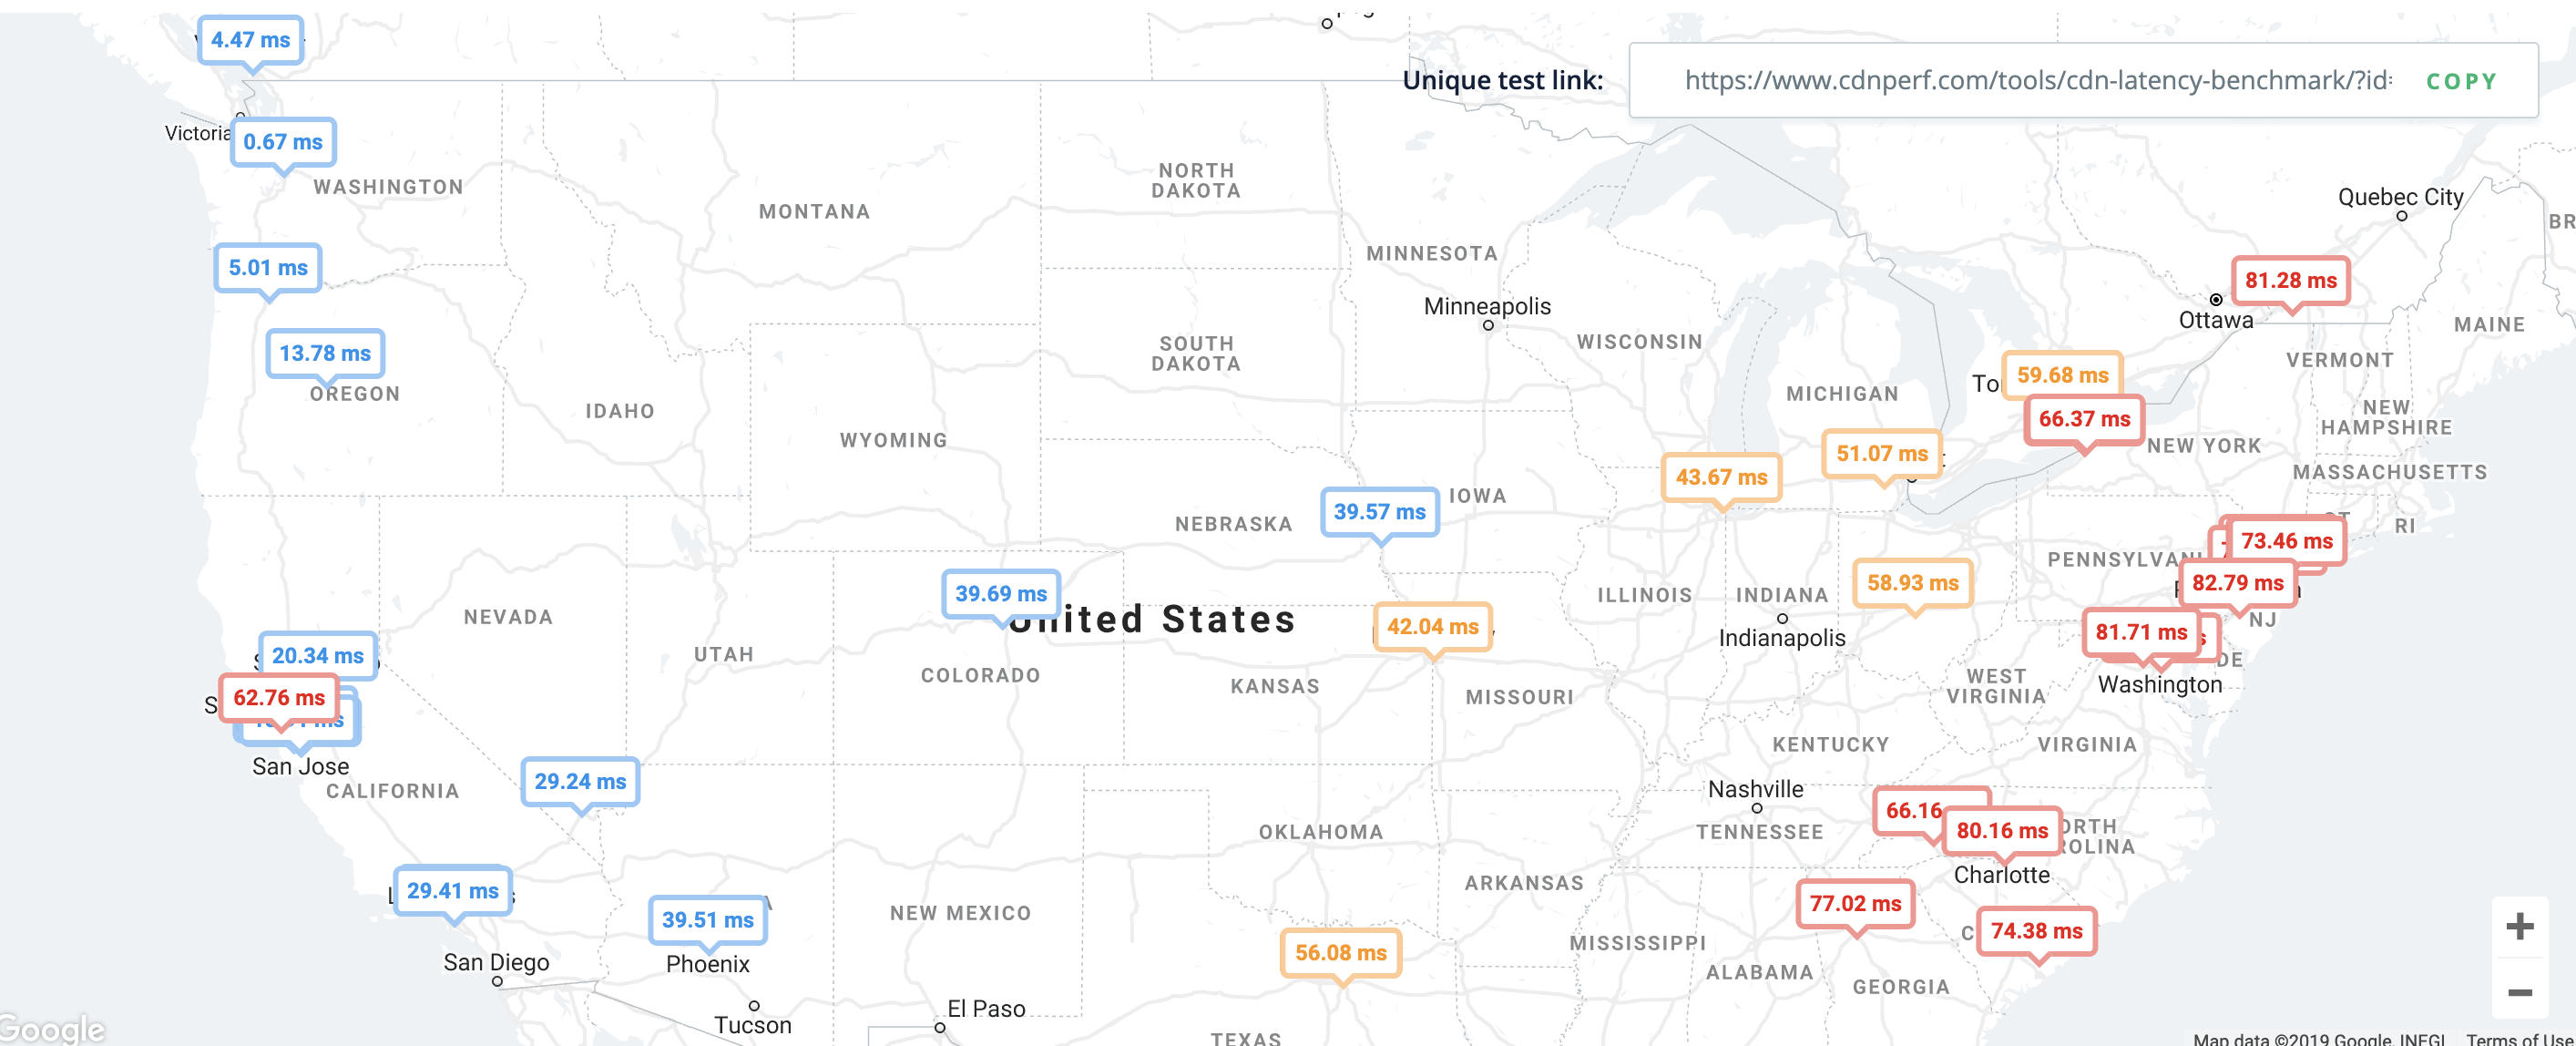
\includegraphics[width=15cm]{11}

      Note how the pings gradually get larger as you move away from Seattle, with
      the shortest ping in the Seattle area.

      Meanwhile the server 99.84.46.77 is most likely in the New York City region
      based on the ping map: \\
      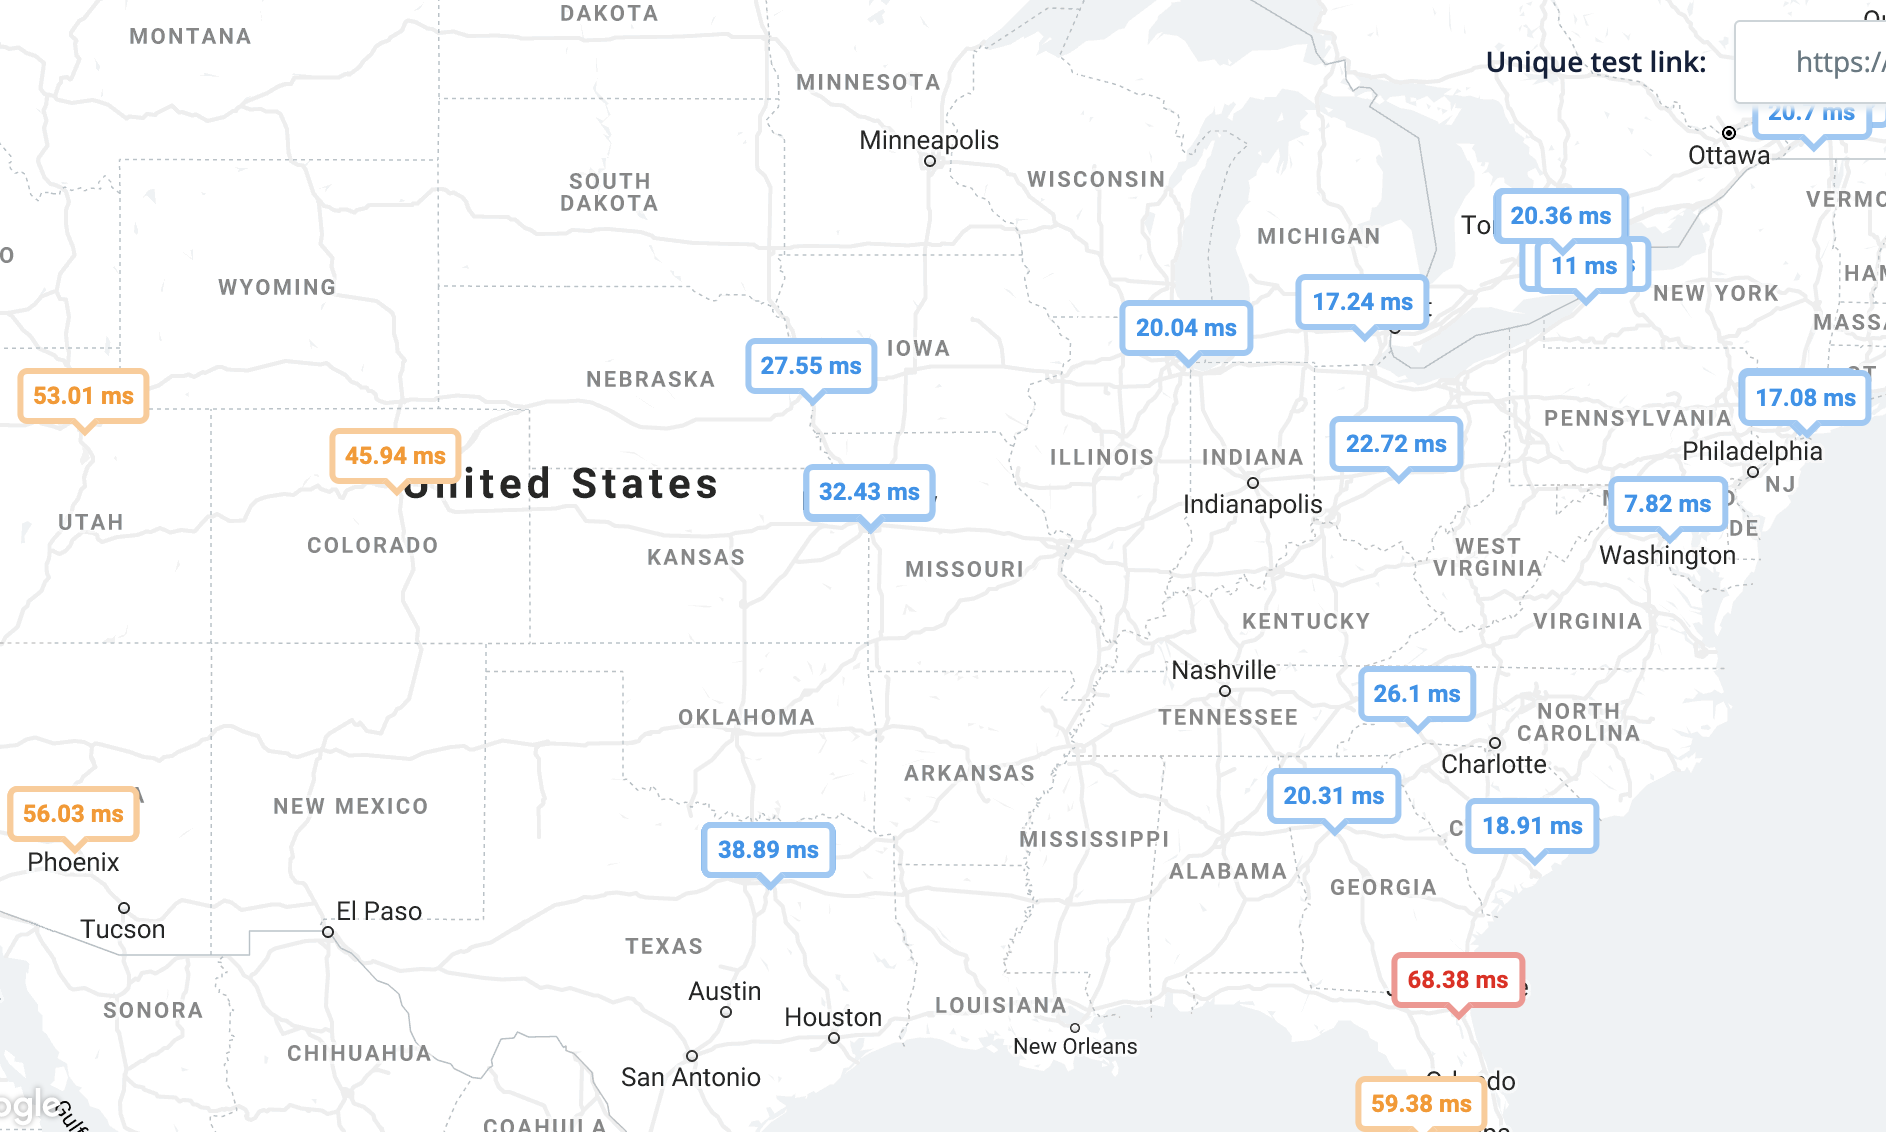
\includegraphics[width=15cm]{12}

      See how the pings gradually become larger as you move away from the New York
      City area. Furthermore, upon closer inspection within NYC: \\
      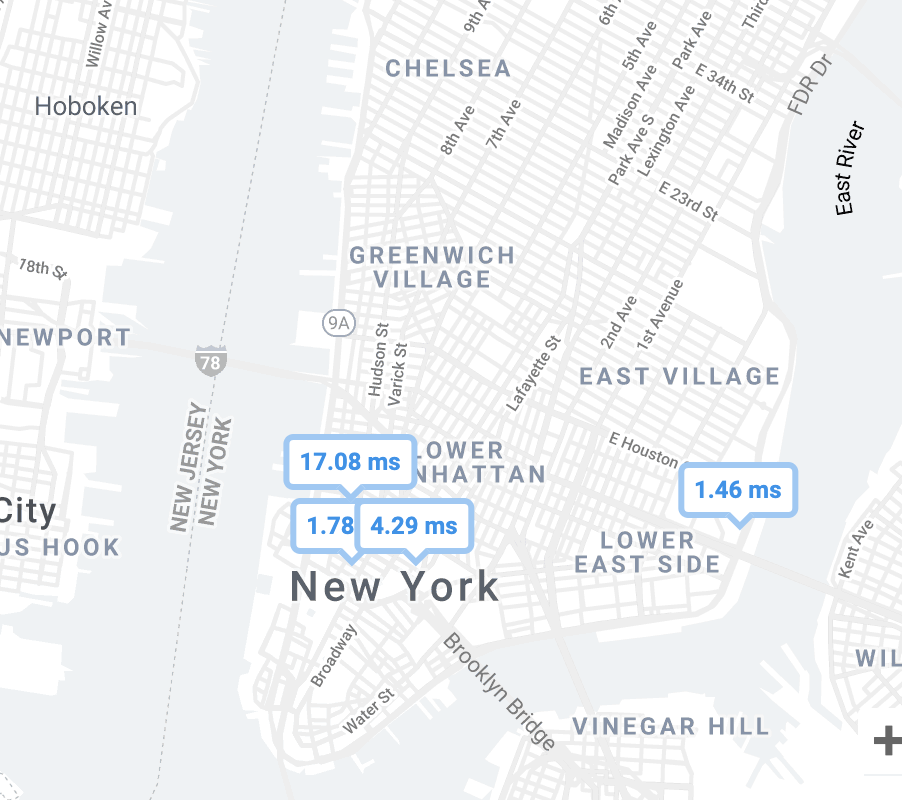
\includegraphics[width=15cm]{13}

      The pings get very small once we are in NYC. This means the server is most
      likely in New York City.
  \end{enumerate}

\section*{Bonjour, Le Monde!}
  \begin{enumerate}[(a)]
    \item The Columbia local DNS server
    \item DNS protocol
    \item UDP
    \item Port 53
    \item UDP is significantly faster since there is no overhead of establishing
          a connection for every client that is trying to resolve a domain name
    \item Smaller packet header overhead with UDP segments
    \item The application protocol does not use conditional requests. It uses TTL
          as an expiration date for the cache instead. This is better because it
          saves the amount of requests that are made to upper level servers.
    \item Local DNS Server -> Root DNS -> .fr TLD DNS server -> lemonde.fr Authoritative DNS server
    \item Yes -- a deployment could exist where the authoritative DNS server is closer
          to the TLD DNS server, which is closer to the root DNS server than
          to the local DNS server.
    \item DNS poisoning may have happened, where an attacker set a bogus redirection
          that is cached within the DNS server
    \item DNS is vulnerable because the local DNS conducts the caching and once
          is set, the false redirection won't change until the cache expires.
  \end{enumerate}

\end{document}
